\documentclass{beamer}

\usepackage[utf8x]{inputenc}
%\usepackage{default}
\usepackage{beamerthemesplit}
\usepackage{tikz}
\usepackage{subfigure}
\usepackage{color}
\usepackage{listings}
\usepackage{graphicx}
\usepackage{amsmath}

\usepackage[ruled]{algorithm2e}
% \usepackage{algorithmic}

\newcounter{saveenumi}
\newcommand{\seti}{\setcounter{saveenumi}{\value{enumi}}}
\newcommand{\conti}{\setcounter{enumi}{\value{saveenumi}}}

\resetcounteronoverlays{saveenumi}

\setbeamertemplate{navigation symbols}{} 

%\setbeamertemplate{footline}[page number]{}
\setbeamertemplate{footline}{}
% \usetheme{Berkeley}
% \usetheme{Antibes}
% \usetheme{Bergen}
% \usetheme{Berlin}
% \usetheme{Boadilla}
% \usetheme{Copenhagen}   %good
    \usetheme{Madrid}   %better
%    \usetheme{Warsaw}   %better



\title[JPass]{PV204: Project Presentation}

\author[RPD]{Rudolf Wittner, Peter Sooky, Deepak  Vishwakarma}
\institute[MU]{Faculty of Informatics, MU}

%\author[DEEPAK]{Deepak Vishwakarma}

%\institute[MU]{Faculty of Informatics, Masaryk University}
\date{May 5th, 2016}

  \begin{document}
  \maketitle


  \begin{frame}
    \frametitle{Overview}
     \begin{itemize}	
      \item JPass: the Opensource application
      \item Applet Design
      \item PC Application
      \item Security Analysis
      \item  Conclusion
     \end{itemize}
  \end{frame}
  
  \begin{frame}
    \frametitle{JPass: the Opensource application}
    \begin{enumerate}
    	\item Password Manager
    	\item \emph{https://github.com/gaborbata/jpass}
	\item Functionalities:
	\begin{enumerate} [-]
		\item Creation/generation of passwords
		\item Organize username, password, URL
		\item Import/Export in XML
		\item User Verification
		\item Change PIN
		\item Save /Open file
	\end{enumerate}	
     \end{enumerate}  
  \end{frame}

  \begin{frame}
    \frametitle{JPass: Features Targeted}
    \begin{enumerate}
    	\item User verification through smart card (PIN)
	\item Password generation in smart card
	\item Storage of passwords in smart card
	\item Other attributes URL, ID can be stored in JPass (secured way)
     \end{enumerate}  
  \end{frame}
  
  \begin{frame}
    \frametitle{Applet Design}
  	\begin{enumerate}
	\item User authentication
	\item Change user PIN
	\item Generate Passwords
	\item Store passwords
	\item Password Retrieval
	\item Update/delete password		
	\end{enumerate}
  \end{frame}
  
  \begin{frame}
    \frametitle{PC Application}
    
    \begin{enumerate}
    	\item User authentication
	\item Change user PIN
	\item Generate passwords request
	\item Save passwords
	\item Retrieve passwords 
	\item Update/delete password	
    \end{enumerate}  
  \end{frame}
  
  \begin{frame}
    \frametitle{Communication Security}
  
  \end{frame}
  
  \begin{frame}
    \frametitle{Attacker Model}
    	\begin{enumerate}
  	\item Listen to the channel
		\begin{enumerate} [$\implies$]		\pause
			\item  \emph{eavesdropping}
		\end {enumerate}
		\pause 
 	\item Collect communication data  \pause 
		\begin{enumerate} [$\implies$]
			\item attacker can learn the \emph{session key} or PIN
		\end {enumerate}
		\pause 
	\item Store and forward data  \pause 
		\begin{enumerate} [$\implies$]
			\item  attacker can launch replay attack
		\end {enumerate}
		\pause 
	\item Modify and send data to the smart card of PC application \pause 
		\begin{enumerate} [$\implies$]
			\item  attacker can try to authenticate to smart card
			\item send arbitrary commands to smart card
			\item  try to get data leaked from pc application or smart card
		\end {enumerate}
	\end {enumerate}
  \end{frame}
  
  \begin{frame}
    \frametitle{Security Mechanism}
    	\centering
  	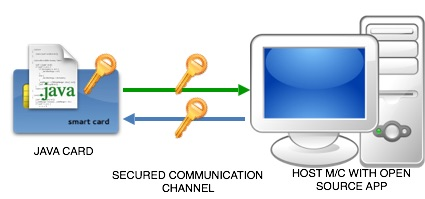
\includegraphics[width=\textwidth]{sample}
  \end{frame}
  
  \begin{frame}
    \frametitle{Security Mechanism:Session Key Derivation}
    	\begin{enumerate}
		\item Session Key Derivation:
			\begin{enumerate}[-]
				\item Generate a salt (random number) in smart card
				\item Session key hash (PIN + random number)
				\item Different session key for every session due to salt
				\item PIN acts as master secret which can be changed based on some policy
			\end{enumerate}
		\item Freshness of data
			\begin{enumerate}[-]
				\item applet and PC application use nonce to ensure it
			\end{enumerate}
	\end{enumerate}
  \end{frame}  
  
  
  \begin{frame}
    \frametitle{Attacker Mittigation}
    	\begin{enumerate}
  	\item Listen to the channel
		\begin{enumerate} [$\implies$]		\pause
			\item  encrypted data
			\item all an attacker see in plain is a random number
		\end {enumerate}
		\pause 
 	\item Collect communication data  \pause 
		\begin{enumerate} [$\implies$]
			\item hard to do as session key is different for every session
		\end {enumerate}
		\pause 
	\item Store and forward data  \pause 
		\begin{enumerate} [$\implies$]
			\item  Nonce used by PC application and applet will protect against this
		\end {enumerate}
		\pause 
	\item Modify and send data to the smart card of PC application \pause 
		\begin{enumerate} [$\implies$]
			\item  Any modification of encrypted data would destroy it and can be rejected
			\item Use HMAC to ensure the integrity of data
		\end {enumerate}
	\end {enumerate}
  \end{frame}
  
  
  \begin{frame}
    \begin{center}
      \huge $\mathcal{THANK ~~~ YOU}$\\ \ \\ \ \\      
    \end{center}
  \end{frame}





\end{document}
